% Exhibits accompanying the presubmission enquiry: the five main figures and the main
% table, with the full captions as they appear in the manuscript.
% Generated by build_supplement_tex.py - edit that script, not this file.
\documentclass[11pt]{article}
\usepackage[a4paper,top=1.6cm,bottom=1.6cm,left=1.5cm,right=1.5cm]{geometry}
\usepackage[T1]{fontenc}
\usepackage{newtxtext}
\usepackage{graphicx}
\usepackage{booktabs}
\usepackage{multirow}
\usepackage{array}
\usepackage{amsmath,amssymb}
\usepackage[numbers,sort&compress]{natbib}
\usepackage{hyperref}
\hypersetup{hidelinks}
\setlength{\parindent}{0pt}
\setlength{\parskip}{0.45em}
\pagestyle{empty}

% the sn-mathphys-num style expects helpers provided by the sn-jnl class
\providecommand{\citeauthoryear}[2]{#1, #2}
\providecommand{\citenum}[1]{#1}
\providecommand{\bibcommenthead}{}

\newcommand{\exhibit}[1]{%
  \par\vspace{0.5em}
  {\footnotesize \textbf{Figure.}~#1}\par
}

\begin{document}

{\footnotesize Supplement to the presubmission enquiry \hfill 22 November 2026}\\[-0.25em]
\rule{\textwidth}{0.4pt}
\vspace{0.5em}

{\bfseries\large Bridging protein and nucleic-acid pockets via shared physicochemical
representations for 3D molecular generation with NA2smol --- main figures and table}

\vspace{0.3em}
{\footnotesize Letian Gao, Yi Li, Wenbiao Zhou, Jiahao Chen, Bing Su, Xing Li and Zhi John Lu}\\[-0.15em]
{\footnotesize \emph{Tsinghua University; Renmin University of China; Institute of Zoology, Chinese Academy of Sciences}}\\[-0.15em]
{\footnotesize Equal contribution: Letian Gao, Yi Li, Wenbiao Zhou and Jiahao Chen. Corresponding authors: Bing Su, Xing Li and Zhi John Lu.}

\vspace{0.8em}
{\footnotesize\emph{This supplement reproduces the five main figures and the main table with the
captions as submitted with the manuscript.}}\par
\vspace{0.4em}
{\footnotesize
\textbf{Figure 1} Workflow, training and candidate prioritisation.\par
\textbf{Figure 2} Paired benchmark evaluation on the DUD-E protein benchmark and the RNA test set.\par
\textbf{Figure 3} Comparison of the four NA2smol training configurations.\par
\textbf{Figure 4} Structure-based design of fluorogenic ligands for the Clivia aptamer.\par
\textbf{Figure 5} Experimental validation of a ligand candidate for the KRAS promoter G-quadruplex.\par
\textbf{Table 1} Metric values for both benchmarks and the four training configurations.\par
}

\clearpage
\section*{Figure 1}
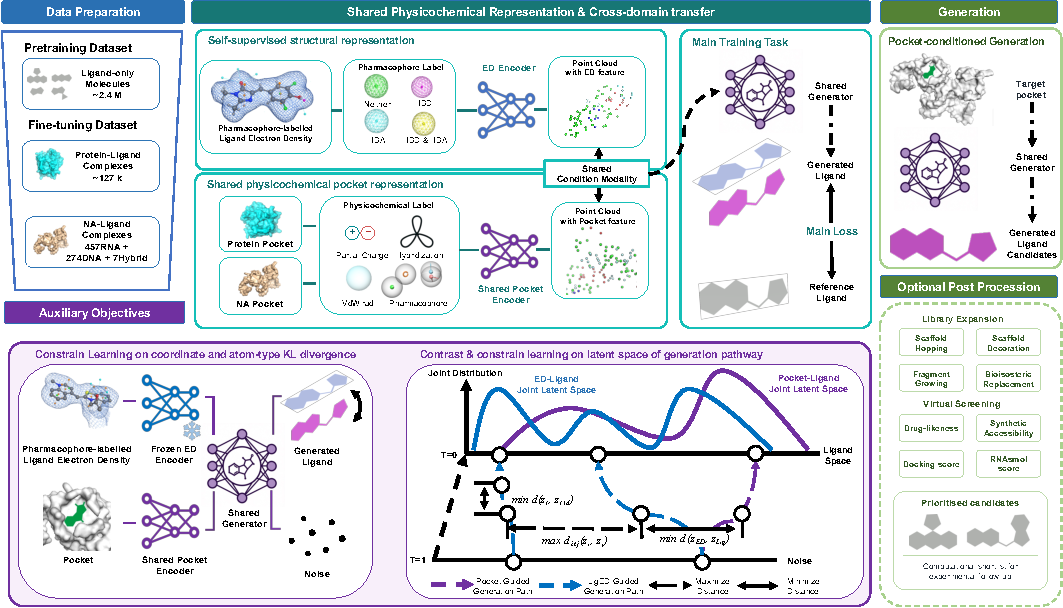
\includegraphics[width=0.98\textwidth,height=0.60\textheight,keepaspectratio]{figures/figure1_nbt.pdf}
\exhibit{Workflow, training and candidate-prioritisation strategy of NA2smol. \textbf{Data preparation} (top left). Pretraining uses a ligand-only library ($\sim$2.4~M molecules) represented as pharmacophore-labelled ligand ED maps. Fine-tuning uses protein--ligand ($\sim$127~k) and nucleic-acid--ligand complexes (738 curated records: 356 training and 382 validation). \textbf{Shared physicochemical representation and cross-domain transfer} (top centre). A self-supervised encoder maps four-class pharmacophore-labelled ligand ED (neither, HBD only, HBA only, or both) to an ED point cloud. In parallel, a shared pocket encoder maps protein or nucleic-acid pockets to a physicochemical point cloud (partial charge, hybridisation, van der Waals radii and pharmacophore label) feeding the shared generator (Methods). \textbf{Auxiliary objectives} (bottom left). Constrained learning on the predicted outputs aligns the pocket-conditioned student with the frozen ED teacher on coordinates and atom-type distributions. Contrastive learning acts on flow states during ED pretraining ($d(z_i,z_{i+\Delta})$ and $d_{\mathrm{iff}}(z_i,z_j)$) and across teacher and student views for the full model during fine-tuning ($d(z_{\mathrm{ED}},z_{\mathrm{lig}})$). \textbf{Generation} (top right). Conditioned on a target pocket, the shared generator produces candidate ligands. \textbf{Optional post-processing} (right). Candidates can undergo library expansion and multi-objective virtual screening (drug-likeness, synthetic accessibility, docking score and RNAsmol score) to prioritise compounds for experimental follow-up. Schematic time $T$ runs opposite to sampling time $t$ in Methods ($T=1-t$). LigED, ligand electron density; NA, nucleic acid; HBD and HBA, hydrogen-bond donor and acceptor; VdW, van der Waals.}

\clearpage
\section*{Figure 2}
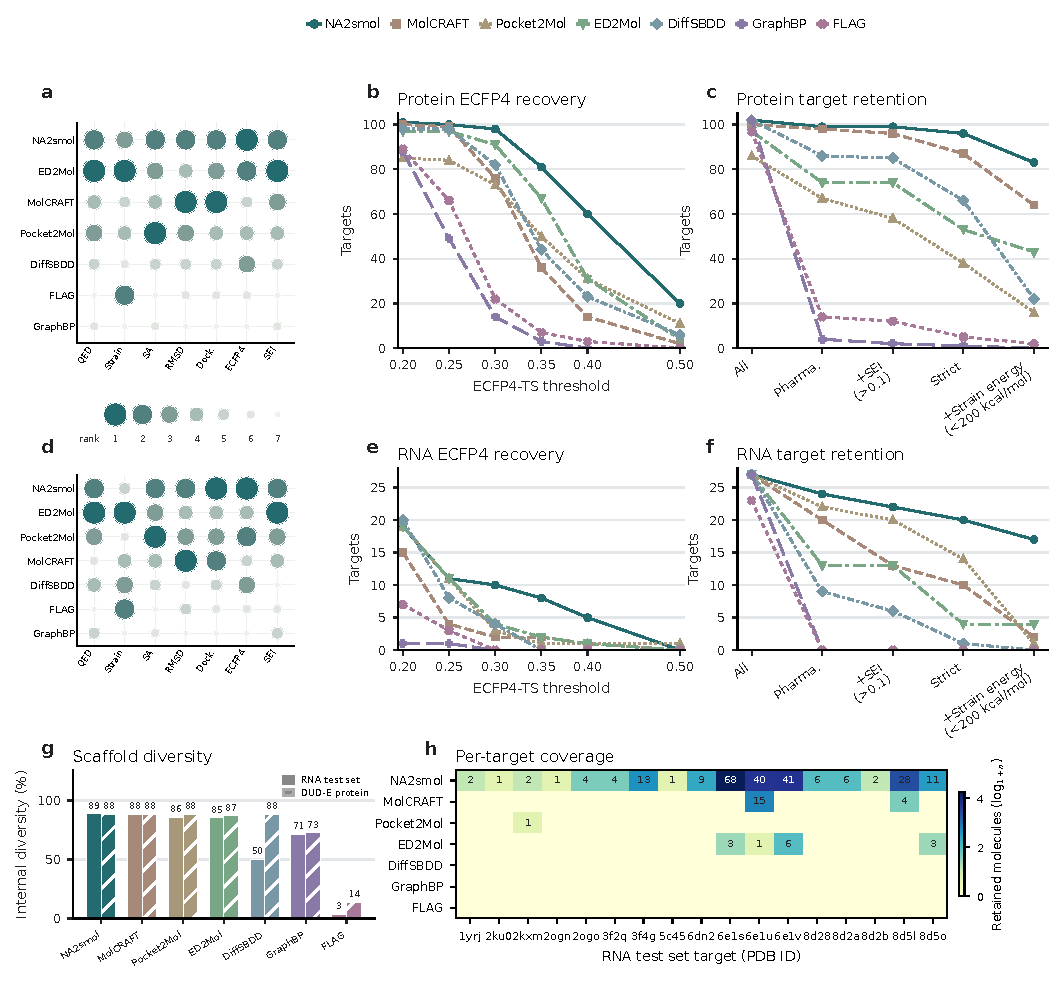
\includegraphics[width=0.98\textwidth,height=0.60\textheight,keepaspectratio]{figures/figure2_nbt.pdf}
\exhibit{Paired benchmark evaluation on the DUD-E protein benchmark and the RNA test set (27 shared evaluable RNA targets). a, DUD-E method-by-metric rank grid across seven axes (Dock., docking score; RMSD after pose relaxation; QED, quantitative estimate of drug-likeness; SA, synthetic accessibility score; SEI, surface efficiency index; ECFP4, extended-connectivity fingerprint similarity; and Strain, conformational strain energy). Bubble diameter and shade encode method rank on each axis from best (largest, darkest) to worst (smallest, palest) across NA2smol and six external generators (MolCRAFT, Pocket2Mol, ED2Mol, DiffSBDD, GraphBP and FLAG). Axis definitions are in Methods, raw medians in Table~1. b, DUD-E reference-ligand recovery over the fixed 101-target reference universe; missing valid output counts as unrecovered, as on the ECFP4 axis in panel a. c, DUD-E screening retention as absolute target counts over method-specific outputs (85--102 targets per method) across the four-tier cascade (Methods). d, RNA test-set method-by-metric rank grid corresponding to panel a. e,f, RNA test-set reference-ligand recovery (e) and screening retention (f) across the 27 shared evaluable targets. g, Internal scaffold diversity: unique Bemis--Murcko \cite{bemis1996} scaffolds as a percentage of each method's distinct generated molecules (solid bars, RNA test set; hatched bars, DUD-E). h, Per-target candidate coverage under the most stringent filter on the RNA test set (retained molecule counts on a logarithmic colour scale).}

\clearpage
\section*{Figure 3}
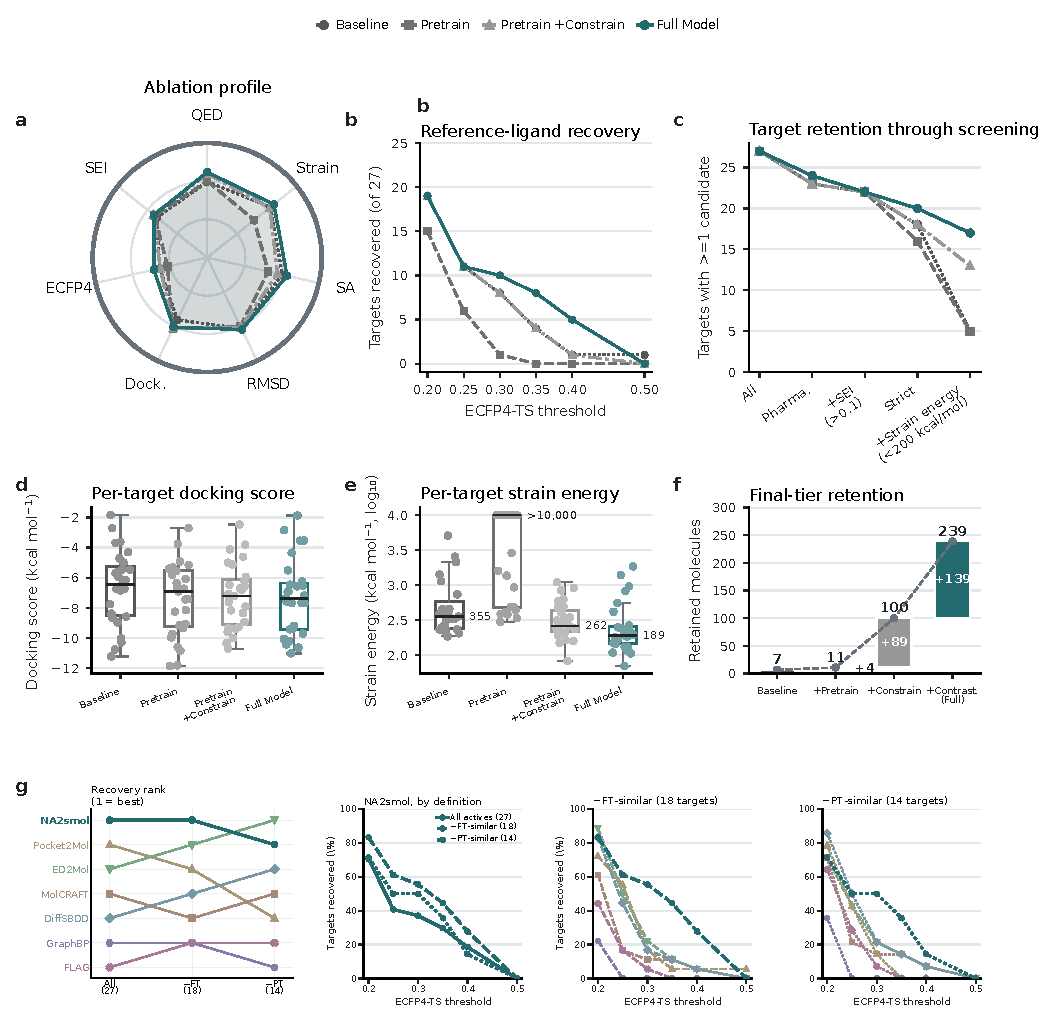
\includegraphics[width=0.98\textwidth,height=0.60\textheight,keepaspectratio]{figures/figure3_nbt.pdf}
\exhibit{Comparison of NA2smol training configurations on the RNA test set (four configurations, $n=27$ targets per configuration). a, Ablation profile across the same seven metrics as Fig.~2d (docking, RMSD, QED, SA, SEI and Strain as retention-curve integrals; ECFP4 recovery as its raw area); a larger radial distance means better performance. b, Reference-ligand recovery: targets with at least one molecule reaching the ECFP4-Tanimoto similarity threshold. c, Targets with at least one retained molecule through the screening cascade. d, Per-target smina docking-score distributions. e, Per-target conformational strain energy (PoseCheck \cite{harris2023posecheck}) on a $\log_{10}$ scale; labels give the median of per-target medians in kcal~mol$^{-1}$, with medians at the $10^{4}$ bound labelled $>10,000$. f, Differences in retained molecule counts between successive configurations (waterfall); bars show incremental gain and the dashed line the cumulative total. g, ECFP4 recovery across similarity-filtered target subsets (four panels): recovery rank of each method on the three target sets (all actives, 27; fine-tuning-similar actives removed, 18; pretraining-library-similar actives removed, 14), with method colours keyed on the left axis and vertical position giving the rank (1 = best); NA2smol recovery curves on the same three target sets; and recovery curves of all seven methods on the fine-tuning-similar-removed and pretraining-similar-removed subsets (fraction of eligible targets with at least one molecule above the ECFP4-Tanimoto similarity threshold). For e, strain values above $10^{4}$~kcal~mol$^{-1}$ and failed evaluations were set to $10^{4}$~kcal~mol$^{-1}$; in d,e, boxes show the interquartile range, centre lines medians and points target-level medians.}

\clearpage
\section*{Figure 4}
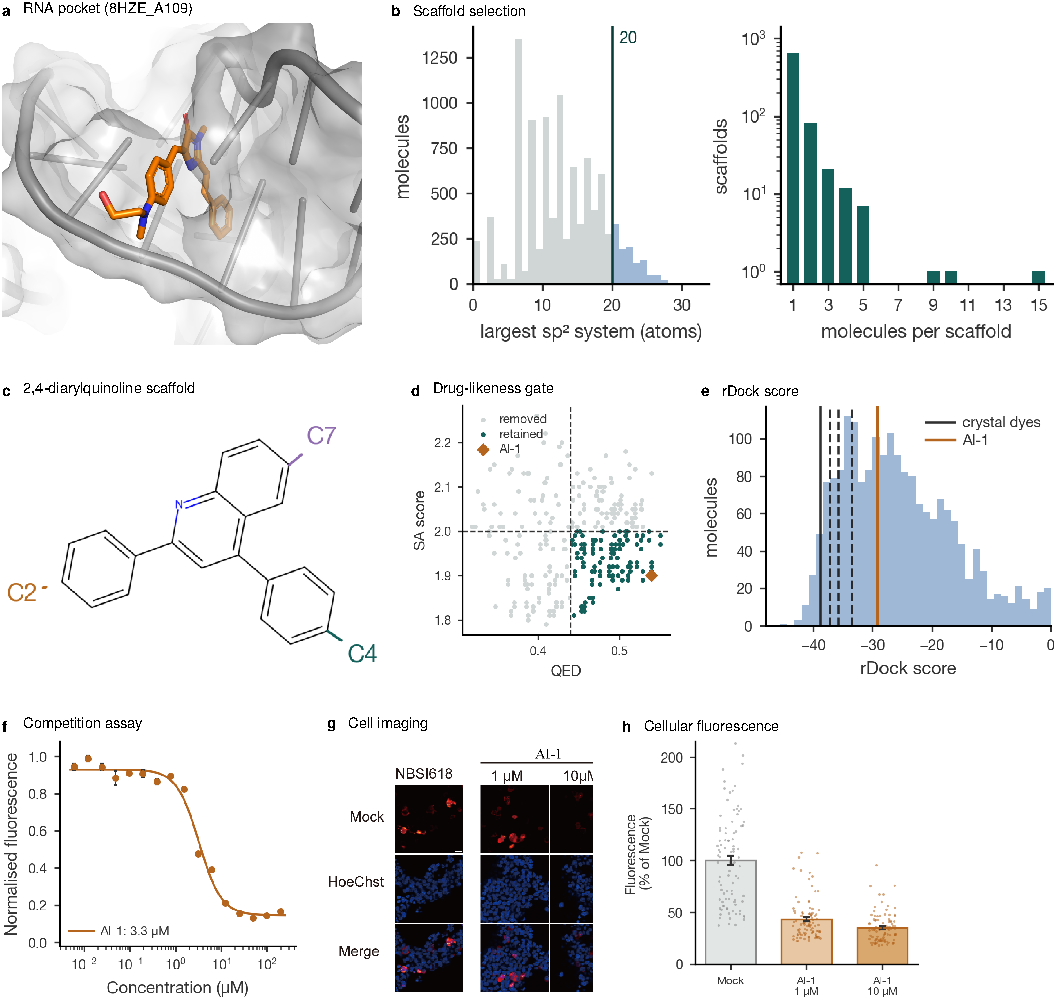
\includegraphics[width=0.98\textwidth,height=0.60\textheight,keepaspectratio]{figures/figure5_clivia.pdf}
\exhibit{Structure-based generative design of fluorogenic ligands for the Clivia aptamer. \textbf{a}, The representative pocket (8HZE\_A109) with the crystal dye NI4; RNA is shown as a cartoon with a semi-transparent molecular surface and the ligand as sticks. \textbf{b}, Scaffold selection. Left: distribution of the largest sp$^{2}$-connected system in the 9,880 closed-shell, neutral generated molecules (grey, below the 20-atom cut; blue, at or above it). Right: distribution of scaffold repetition among the retained molecules (996 molecules, 777 scaffolds); most scaffolds occur once, and the most frequent scaffold occurs 15 times. \textbf{c}, Substitution positions and substituent vocabulary. Left: the 2,4-diarylquinoline core with the three variable positions marked (C4-aryl para, C2-aryl para, quinoline C7). Right: number of molecules carrying each substituent at each position, counted over the 4,948 products that retained the intact three-ring system. \textbf{d}, Al-1 (orange) and Al-2 (purple) in the binding pocket, in the poses used for scoring. \textbf{e}, QED versus SA score for the 448 molecules (dashed lines, QED $=0.44$ and SA $=2.00$); 198 molecules are retained (teal), and Al-1 and Al-2 are marked. \textbf{f}, Distribution of the in-place-minimised rDock score across the 1,908 scored molecules of the reference enumeration; the four crystal dyes (black; NI4 $=-38.9$) and Al-1/Al-2 are marked. \textbf{g}, Competition dose--response for Al-1 and Al-2 (points, mean $\pm$ SD; lines, four-parameter logistic fits). \textbf{h}, Representative confocal images of Clivia-aptamer-expressing cells treated with Al-1 or Al-2 (NBSI618 channel, Hoechst nuclear stain, merge); Mock, untreated. \textbf{i}, Quantification of cellular fluorescence from \textbf{h} (93 cells per condition; bars, mean; error bars, SEM; dots, individual cells; percentage of the Mock mean).}

\clearpage
\section*{Figure 5}
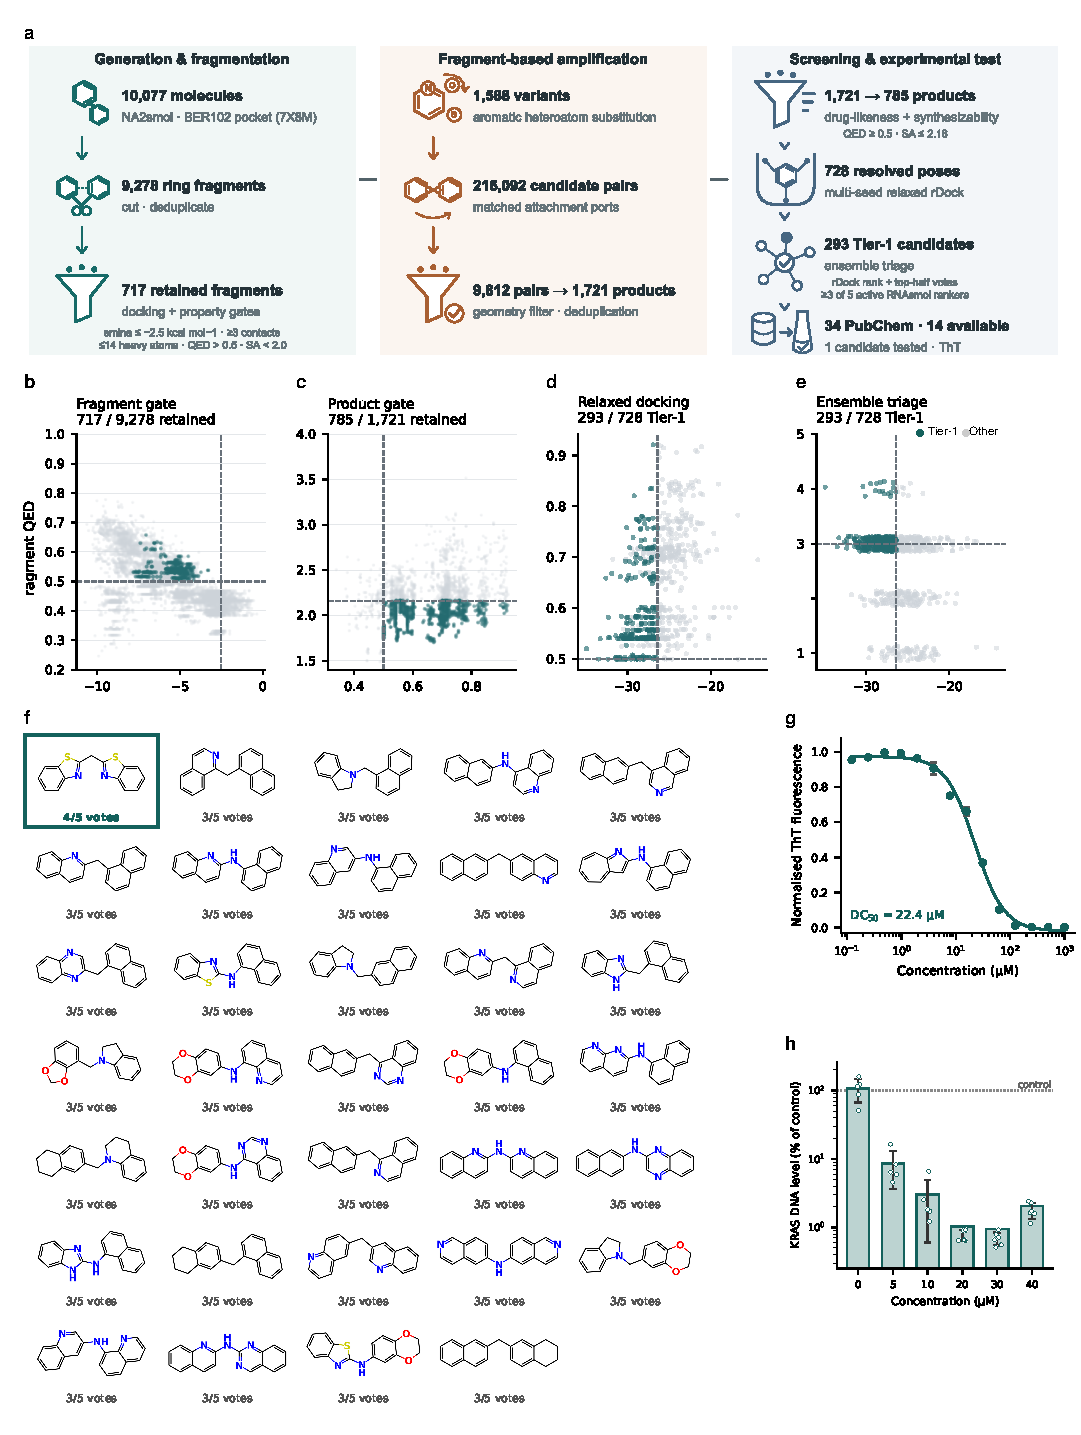
\includegraphics[width=0.98\textwidth,height=0.60\textheight,keepaspectratio]{figures/figure5_kras.pdf}
\exhibit{Experimental validation of an NA2smol-derived ligand candidate for the KRAS promoter G-quadruplex. \textbf{a}, NA2smol generation at the BER102 site (7X8M), post-processing, candidate prioritisation and experimental testing. \textbf{b}, Fragment gate: smina score versus QED across pooled ring fragments (dashed lines: $-2.5$~kcal~mol$^{-1}$ and QED $=0.5$; additional gates in Methods). \textbf{c}, Product gate: QED versus SA across assembled products (dashed lines: QED $=0.5$ and SA $=2.16$). Teal denotes retained molecules in \textbf{b},\textbf{c}. \textbf{d}, Relaxed rDock score versus QED across dock-resolved products; Tier-1 candidates are teal and others grey. Dashed lines mark the rDock median and QED $=0.5$. \textbf{e}, RNAsmol votes versus rDock score; the dashed line marks three votes and vertical jitter is used. \textbf{f}, PubChem-recorded Tier-1 candidates ordered by votes (descending), rDock (ascending) and CID, drawn at uniform bond length and labelled with their vote count out of five. The framed structure is candidate 01 (CID 74755, four votes), which was tested experimentally; the others have three votes. \textbf{g}, ThT fluorescence response for candidate 01 with a four-parameter logistic fit; points and error bars show means and SDs from three independent measurements per concentration. \textbf{h}, KRAS DNA level measured by quantitative PCR on a logarithmic scale after treatment with the indicated concentrations of candidate 01, with GAPDH as internal reference (bars, mean; error bars, SD; open circles, individual replicates; $n=5$--$6$ from two independent experiments, normalised to the untreated control; dotted line, 100\% control level).}

\clearpage
\section*{Table 1}
\begin{table}[!htbp]
\centering
\scriptsize
\renewcommand{\arraystretch}{0.94}
\setlength{\tabcolsep}{1.6pt}
\begin{tabular}{@{}lcccccccc@{}}
\toprule
\textbf{Method} & \textbf{Dock.} & \textbf{RMSD} & \textbf{QED} & \textbf{SA} & \textbf{SEI} & \textbf{Strain} & \textbf{Rec.} & \textbf{Top-2 $\uparrow$} \\
\midrule
\multicolumn{9}{@{}l}{\textit{DUD-E protein benchmark}} \\
NA2smol & \underline{$-8.19$} & \underline{0.87} & \underline{0.647} & 3.14 & \underline{0.114} & 130 (95\%) & \textbf{0.656} & \textbf{5/7} \\\\
ED2Mol & $-6.06$ & 1.87 & \textbf{0.736} & \underline{3.04} & \textbf{0.128} & \textbf{26} (97\%) & \underline{0.482} & \textbf{5/7} \\\\
MolCRAFT & $\mathbf{-9.86}$ & \textbf{0.38} & 0.527 & 4.11 & 0.106 & 259 (93\%) & 0.331 & \underline{2/7} \\\\
Pocket2Mol & $-5.89$ & 1.47 & 0.565 & \textbf{3.00} & 0.092 & 218 (97\%) & 0.417 & 1/7 \\\\
FLAG & $-3.86$ & 3.25 & 0.400 & 6.57 & 0.043 & \underline{30} (96\%) & 0.142 & 1/7 \\\\
DiffSBDD & $-5.47$ & 2.79 & 0.493 & 5.67 & 0.057 & 337 (82\%) & 0.457 & 0/7 \\\\
GraphBP & $-1.33$ & 4.45 & 0.481 & 6.37 & 0.014 & $>10^{4}$ (29\%) & 0.093 & 0/7 \\\\
\midrule
\multicolumn{9}{@{}l}{\textit{RNA test set}} \\
NA2smol & $\mathbf{-7.27}$ & \underline{1.12} & \underline{0.641} & 3.53 & \underline{0.103} & 220 (92\%) & \textbf{0.218} & \textbf{5/7} \\\\
ED2Mol & $-5.16$ & 1.62 & \textbf{0.699} & \textbf{2.85} & \textbf{0.116} & \underline{24} (98\%) & 0.077 & \underline{4/7} \\\\
MolCRAFT & \underline{$-6.91$} & \textbf{0.39} & 0.421 & 3.84 & 0.062 & 125 (97\%) & 0.059 & 2/7 \\\\
Pocket2Mol & $-5.86$ & 1.32 & 0.554 & \underline{2.94} & 0.070 & 380 (71\%) & \underline{0.080} & 2/7 \\\\
FLAG & $-3.52$ & 3.10 & 0.377 & 6.54 & 0.044 & \textbf{9} (95\%) & 0.015 & 1/7 \\\\
DiffSBDD & $-2.95$ & 4.36 & 0.458 & 5.57 & 0.038 & 49 (94\%) & 0.080 & 0/7 \\\\
GraphBP & $-2.37$ & 4.33 & 0.460 & 6.42 & 0.045 & $>10^{4}$ (35\%) & 0.004 & 0/7 \\\\
\midrule
\multicolumn{9}{@{}l}{\textit{RNA test set, four NA2smol configurations}} \\
NA2smol & $\mathbf{-7.27}$ & \underline{1.12} & \textbf{0.641} & \textbf{3.53} & \underline{0.103} & \textbf{220} (92\%) & \textbf{0.218} & \textbf{7/7} \\\\
Pretrain+Constrain & \underline{$-7.21$} & 1.26 & \underline{0.619} & 4.35 & \textbf{0.104} & \underline{290} (84\%) & 0.132 & \underline{4/7} \\\\
Baseline & $-6.03$ & \textbf{1.09} & 0.484 & \underline{3.86} & 0.078 & 380 (91\%) & \underline{0.141} & 3/7 \\\\
Pretrain Only & $-7.19$ & 1.32 & 0.509 & 5.11 & 0.096 & $>10^{4}$ (46\%) & 0.035 & 0/7 \\\\
\bottomrule
\end{tabular}
\caption{Metric values for the DUD-E protein benchmark, the RNA test set and the four NA2smol training configurations. Values are pooled medians over all of a method's molecules. For Strain, values above $10^{4}$~kcal~mol$^{-1}$ and unevaluable geometries are set to $10^{4}$~kcal~mol$^{-1}$ before taking the median; medians reaching this bound are reported as $>10^{4}$~kcal~mol$^{-1}$. Parenthetical values give the percentage of molecules with a successfully evaluated strain at or below this bound. \textbf{Bold} marks the best value in each benchmark group and \underline{underline} the second best; better is lower for Dock., RMSD, SA and Strain, and higher for QED, SEI and Rec. The Top-2 column counts how many of the seven metrics a method ranks first or second on within its group; it uses the same emphasis and orders the rows.}
\label{radar_values_tab}
\end{table}


\clearpage
\bibliographystyle{bst/sn-mathphys-num}
\bibliography{sn-bibliography}

\end{document}
